\documentclass[12pt,a4paper,oneside]{book}
% --- CONFIGURAZIONE OTTIMIZZATA PER APPUNTI DI INGEGNERIA DEL SOFTWARE ---

% 1. Lingua e Codifica
\usepackage[T1]{fontenc}
\usepackage[utf8]{inputenc}
\usepackage[italian]{babel}

% 2. Layout e Geometria (Sostituisce tutti i calcoli manuali)
\usepackage[a4paper]{geometry}
\geometry{top=2.5cm, bottom=2.5cm, left=2.5cm, right=2.5cm, headheight=15pt}
\usepackage{parskip} % Gestisce lo spazio tra i paragrafi senza indentazione

% 3. Grafica e Colori
\usepackage{graphicx}
\usepackage{xcolor}
\definecolor{codegreen}{rgb}{0,0.6,0}
\definecolor{codegray}{rgb}{0.5,0.5,0.5}
\definecolor{codepurple}{rgb}{0.58,0,0.82}
\definecolor{backcolour}{rgb}{0.95,0.95,0.92}
\definecolor{unict_blue}{RGB}{0,39,75}

% 4. Codice (Essenziale per Informatica)
\usepackage{listings}
\lstset{
    backgroundcolor=\color{backcolour},   
    commentstyle=\color{codegreen},
    keywordstyle=\color{magenta},
    numberstyle=\tiny\color{codegray},
    stringstyle=\color{codepurple},
    basicstyle=\ttfamily\small,
    breakatwhitespace=false,         
    breaklines=true,                 
    captionpos=b,                    
    keepspaces=true,                 
    numbers=left,                    
    numbersep=5pt,                  
    showspaces=false,                
    showstringspaces=false,
    showtabs=false,                  
    tabsize=2,
    language=SQL % Default per il tuo corso
}

% 5. Matematica e Simboli
\usepackage{amsmath, amssymb, amsthm, bm}
\usepackage{pgfplots}
\pgfplotsset{compat=1.18} % Risolve il warning che vedevi

% 6. Intestazioni e Pié di pagina (Fancyhdr pulito)
\usepackage{fancyhdr}
\pagestyle{fancy}
\fancyhf{} % Pulisce tutto
\fancyhead[L]{\nouppercase{\leftmark}} % Capitolo a sinistra
\fancyhead[R]{\thepage} % Numero pagina a destra
\renewcommand{\headrulewidth}{0.4pt}


% 7. Ambienti per Definizioni (Belli da vedere)
\usepackage[most]{tcolorbox}
\newtcbtheorem[number within=chapter]{definition}{Definizione}{
    enhanced, % <--- FONDAMENTALE PER RENDERIZZARE IL TITOLO ESTERNO
    colback=unict_blue!5,
    colframe=unict_blue,
    coltitle=white, % <--- TESTO BIANCO PER LEGGIBILITA'
    fonttitle=\bfseries,
    separator sign={:},
    boxrule=0.5pt,
    attach boxed title to top left={yshift=-2mm, xshift=2mm},
    boxed title style={colback=unict_blue}
}{def}

% 8. Altri pacchetti utili
\usepackage{enumitem}
\usepackage{hyperref} % Link cliccabili nell'indice
\hypersetup{
    colorlinks=true,
    linkcolor=unict_blue,
    filecolor=magenta,      
    urlcolor=cyan,
    pdftitle={Appunti Ingegneria del Software},
}
\usepackage{tikz}
\usetikzlibrary{positioning}
\usepackage{float}


\title{Reti di Calcolatori}
\author{Michela Maria Tasca \\ \small Prof. Rundo --- UniCt}
\date{A.A. 2025/2026}

\begin{document}

\maketitle
\tableofcontents

\chapter{Introduzione alle Reti di Calcolatori}

\section{Struttura e Componenti di una Rete}

\begin{definition}{Rete Informatica}{}
Una rete informatica è un sistema che permette il collegamento e la comunicazione tra più dispositivi indipendenti.
\end{definition}

Un sistema di comunicazione si compone fondamentalmente di due dimensioni interconnesse:

\begin{itemize}
    \item \textbf{Parte Fisica}: Costituita dall'infrastruttura hardware che connette i dispositivi. I nodi sono collegati tramite \textbf{communication link} (collegamenti di comunicazione) e \textbf{packet switch} (commutatori di pacchetto).
    \begin{itemize}
        \item \textbf{Mezzi fisici}: I collegamenti possono utilizzare cavi di rame, fibre ottiche o onde elettromagnetiche.
        \item \textbf{Velocità di trasmissione}: Viene misurata in \textbf{bps} (bit per secondo).
    \end{itemize}
    \item \textbf{Parte Logica}: Rappresenta l'insieme di regole e software che permettono la trasmissione e la ricezione dei dati attraverso il mezzo fisico.
\end{itemize}

\subsection{Commutazione di Pacchetto e Instradamento}
Nelle reti moderne, le informazioni non vengono inviate come un unico flusso continuo, ma vengono divise in unità più piccole chiamate \textbf{pacchetti}.

\begin{itemize}
    \item \textbf{Composizione del Pacchetto}: Ad ogni frammento di dati viene aggiunta un'\textbf{intestazione} (header) contenente informazioni di controllo.
    \item \textbf{Packet Switch}: Dispositivi come \textbf{router} o \textbf{link layer switch} ricevono i pacchetti su un collegamento in ingresso e li inoltrano su uno in uscita.
    \item \textbf{Route (Percorso)}: La sequenza di collegamenti e commutatori attraversati da un pacchetto dalla sorgente alla destinazione.
    \item \textbf{Accesso alla Rete}: Gli utenti accedono a Internet tramite gli \textbf{ISP} (Internet Service Provider).
\end{itemize}

\subsection{Protocolli di Comunicazione}

\begin{definition}{Protocollo}{}
Un protocollo definisce il formato e l'ordine dei messaggi scambiati tra due o più entità in comunicazione, specificando le azioni da intraprendere durante la trasmissione, la ricezione o in risposta a determinati eventi.
\end{definition}

I due protocolli fondamentali dell'architettura Internet sono il \textbf{TCP} (Transmission Control Protocol) e l'\textbf{IP} (Internet Protocol). Lo sviluppo degli standard è affidato alla \textbf{IETF} (Internet Engineering Task Force), che pubblica i dettagli tecnici tramite i documenti \textbf{RFC} (Request For Comment).

\subsection{Architettura a Livelli ed Incapsulamento}

Per gestire la complessità della progettazione hardware e software, le reti sono strutturate in \textbf{livelli} (layer). Questo approccio modulare facilita l'aggiornamento dei componenti senza dover modificare l'intero sistema.

\subsection{La Pila dei Protocolli (Stack)}
La gerarchia standard si compone di 5 livelli principali:

\begin{enumerate}
    \item \textbf{Livello di Applicazione}: Sede delle applicazioni di rete (es. browser, email).
    \item \textbf{Livello di Trasporto}: Gestisce il trasferimento dei messaggi applicativi tra gli endpoint.
    \item \textbf{Livello di Rete}: Responsabile del trasferimento dei pacchetti (datagrammi) da un host all'altro attraverso la rete.
    \item \textbf{Livello di Collegamento (Data Link)}: Gestisce l'instradamento dei frame tra nodi adiacenti della rete.
    \item \textbf{Livello Fisico}: Si occupa della trasmissione dei singoli bit sul mezzo fisico.
\end{enumerate}

\subsection{Il Concetto di Incapsulamento}
L'incapsulamento è il processo mediante il quale ogni livello aggiunge informazioni di controllo ai dati provenienti dal livello superiore.

\begin{itemize}
    \item \textbf{Payload}: Il carico di dati utile ricevuto dal livello precedente.
    \item \textbf{Header}: Un pre-dato di formattazione che prepara il ricevitore alla gestione dell'informazione successiva.
\end{itemize}

\textbf{Processo di trasmissione (Origine):}
\begin{itemize}
    \item \textbf{Messaggio (M)}: Generato al livello Applicazione.
    \item \textbf{Segmento}: Il livello Trasporto aggiunge l'header $H_t$ (necessario per la consegna alla corretta istanza applicativa).
    \item \textbf{Datagramma}: Il livello Rete aggiunge l'header $H_n$ (per l'instradamento tra host).
    \item \textbf{Frame}: Il livello Collegamento aggiunge l'header $H_l$ (per la consegna fisica tra nodi).
\end{itemize}


\section{Modelli di Riferimento: ISO/OSI e TCP/IP}

\subsection{Il Modello ISO/OSI}
È un modello teorico di riferimento costituito da 7 livelli:
\begin{itemize}
    \item \textbf{Host Layers} (Gestione end-to-end): Application, Presentation (rappresentazione e cifratura dati), Session (comunicazione inter-host), Transport.
    \item \textbf{Media Layers} (Gestione del transito): Network, Data Link, Physical.
\end{itemize}

\subsection{Il Modello TCP/IP}
Utilizzato nelle implementazioni reali, semplifica la struttura in 4 livelli:
\begin{itemize}
    \item \textbf{Application Layer}: Accorpa i livelli Application, Presentation e Session dell'OSI.
    \item \textbf{Transport Layer}: Gestisce la connessione tra processi.
    \item \textbf{Network Layer}: Gestisce l'indirizzamento logico (IP).
    \item \textbf{Network Access Layer}: Accorpa i livelli Data Link e Physical (gestione del mezzo fisico e indirizzamento MAC).
\end{itemize}

\section{Comunicazione e Segnali}

\subsection{Trasmissione Fisica}
I dati sono processati dalle CPU in linguaggio binario. La distinzione tra 0 e 1 avviene tramite soglie di tensione:
\begin{itemize}
    \item \textbf{Bit 1}: Tensione $> 3.3V$.
    \item \textbf{Bit 0}: Tensione $< 0.8V$.
    \item \textbf{Area Intermedia}: Zona di incertezza da evitare per prevenire errori di interpretazione.
\end{itemize}

\textbf{Problematiche del segnale:}
\begin{itemize}
    \item \textbf{Distorsione}: Causata dalla distanza di propagazione e dai ritardi di induzione del mezzo fisico.
    \item \textbf{Ritardo di commutazione}: Il segnale non può cambiare stato istantaneamente da 0 a 1.
\end{itemize}

\subsection{Tipologie di Connessione}
\begin{itemize}
    \item \textbf{Connectionless}: Invio dei dati senza previa instaurazione di una connessione e senza conferma di ricezione (es. invio di una lettera ordinaria).
    \item \textbf{Connection-oriented}: Prevede segnali di \textbf{ACK} (Acknowledge) per confermare la corretta ricezione.
    \item \textbf{Affidabilità}: Necessaria in ambiti critici (medico, militare). Si ottiene spesso tramite il \textbf{Timing}: se un ACK non arriva entro un tempo limite, il dato viene reinviato.
\end{itemize}

\section{Topologie e Classificazione delle Reti}

\subsection{Tipologie di Trasmissione}
\begin{itemize}
    \item \textbf{Point-to-Point}: Comunicazione diretta tra due dispositivi.
    \item \textbf{Broadcast}: Un dispositivo invia segnali a tutti i dispositivi della rete. Richiede la gestione delle \textbf{collisioni}.
\end{itemize}

\subsection{Topologie Fisiche}
\begin{itemize}
    \item \textbf{Bus}: Semplice per il broadcast, ma richiede \textbf{arbitri di bus} per gestire le collisioni se più sistemi trasmettono contemporaneamente.
    \item \textbf{Anello}: Richiede la definizione di un orientamento per la circolazione del segnale.
    \item \textbf{Stella}: I nodi sono collegati a un centro comune; la gestione di più pacchetti avviene tramite temporizzazione.
\end{itemize}

\subsection{Classificazione per Estensione Geografica}
\begin{itemize}
    \item \textbf{PAN} (Personal Area Network): Raggio $\sim 1$ metro.
    \item \textbf{LAN} (Local Area Network): Raggio fino a $1$ km.
    \item \textbf{MAN} (Metropolitan Area Network): Raggio fino a $10$ km.
    \item \textbf{WAN} (Wide Area Network): Raggio da $100$ a $1000$ km.
    \item \textbf{Internet}: WAN planetaria con raggio di circa $10000$ km.
\end{itemize}

\section{Sicurezza nelle Reti}

Le architetture distribuite sono soggette a diverse minacce:

\begin{itemize}
    \item \textbf{Malware}: 
    \begin{itemize}
        \item \textbf{Virus}: Oggetti dannosi legati a file eseguibili.
        \item \textbf{Worm}: Software in grado di autoreplicarsi tra computer.
        \item \textbf{Botnet}: Reti di calcolatori compromessi controllate da remoto.
    \end{itemize}
    \item \textbf{Attacchi di Rete}:
    \begin{itemize}
        \item \textbf{DoS (Denial of Service)}: Esaurimento delle risorse per rendere un servizio indisponibile.
        \item \textbf{Packet Sniffing}: Intercettazione dei pacchetti in transito.
        \item \textbf{IP Spoofing}: Falsificazione dell'indirizzo IP mittente.
    \end{itemize}
\end{itemize}

\chapter{Application Layer}

Il livello di applicazione modella le applicazioni di rete e le modalità di comunicazione tra le varie strutture che compongono il sistema. In questo contesto, la comunicazione avviene tra processi eseguiti su calcolatori diversi (nodi della rete).\\
È  il livello più alto nello stack dei protocolli, ed è quello più vicino all’utente. È infatti il livello delle \textbf{applicazioni di rete}: la vastità delle funzionalità offerte dalle reti, sono alla base del successo di Internet.

\section{Paradigmi di Architettura di Rete}

Le applicazioni di rete si basano principalmente su due paradigmi organizzativi per gestire l'interazione tra gli host:

\subsection{Architettura Client-Server}

Nell'architettura \textbf{Client-Server}, i ruoli dei nodi sono ben definiti e asimmetrici:

\begin{itemize}
    \item \textbf{Server}:
    \begin{itemize}
        \item È un host \textbf{sempre attivo} e connesso alla rete che risponde alle richieste del client
        \item Possiede un \textbf{indirizzo IP statico} (permanente) per facilitare la reperibilità da parte dei client.
        \item Può essere costituito da un singolo calcolatore o da un intero \textbf{data center} scalabile.
        \item \textbf{Sicurezza}: L'IP statico è vulnerabile ad attacchi diretti una volta scoperto.
    \end{itemize}
    \item \textbf{Client}:
    \begin{itemize}
        \item Manda richieste al server
        \item Si connette al server solo quando necessita di un servizio.
        \item Può avere un \textbf{indirizzo IP dinamico}.
        \item I client non comunicano mai direttamente tra loro in questo modello.
    \end{itemize}
\end{itemize}

Esempi di protocolli che utilizzano questo paradigma sono \textbf{HTTP} (web), \textbf{IMAP} (email) e \textbf{FTP} (trasferimento file). In particolare, IMAP permette la visualizzazione delle email memorizzate sul server senza scaricarle localmente, garantendo la sincronizzazione ma rendendo l'utente dipendente dalla disponibilità del server.

\subsection{Architettura Peer-to-Peer (P2P)}

Nell'architettura \textbf{Peer-to-Peer}, il sistema sfrutta la comunicazione diretta tra coppie di host chiamati \textbf{peer}.

\begin{itemize}
    \item ogni client (\textbf{peer}) ha lo stesso ruolo e stesse capacità
    \item \textbf{Assenza di un arbitro}: Non esiste un server centrale che coordina le comunicazioni.
    \item \textbf{Scalabilità intrinseca}: Ogni nuovo peer che entra nella rete apporta nuove risorse, aumentando la capacità di servizio del sistema senza costi eccessivi di infrastruttura.
    \item \textbf{Svantaggi}: Può causare congestione della rete globale (occupazione di banda) e presenta maggiori rischi di sicurezza, poiché i peer possono essere insicuri o malevoli.
\end{itemize}

Esempi tipici sono il file sharing P2P e i protocolli come \textbf{BitTorrent}.

\section{Comunicazione tra Processi}

Sebbene si parli spesso di comunicazione tra host, a livello logico sono i \textbf{processi} in esecuzione sugli host a scambiarsi messaggi.\\
La comunicazione può avvenire:
\begin{itemize}
    \item \textbf{intra-host:} quando due processi risiedono sullo stesso host utilizzano meccanismi di \textbf{Inter-Process Communication IPC} forniti dal sistema operativo. Questi mecccanismi sono altamente efficenti perchè non richiedono l'uso della rete.
    \item \textbf{inter-host:} quando i processi si trovano su host diversi, la comunicazione avviene tramite \textbf{scambio di messaggi} attraverso la rete. Questi messaggi sono solitamente incapsulati in protocolli di livello applicativo (HTTP, SMTP, FTP, ecc) e vengono trasportati tramite protocolli di livello inferiore (TCP; UDP). Lo scambio di messaggi serve a:
    \begin{itemize}
        \item trasferire dati, banalmente
        \item sincronizzare i processi, ovvero a coordinare le azioni nel tempo
    \end{itemize}
\end{itemize}

Perché la comunicazione avvenga correttamente, ogni processo deve essere identificabile univocamente tramite due parametri:
\begin{enumerate}
    \item \textbf{Indirizzo IP}: Identifica l'host (calcolatore) sulla rete (32 bit per IPv4, 128 bit per IPv6).
    \item \textbf{Numero di Porta}: Identifica lo specifico servizio o processo all'interno dell'host.
\end{enumerate}

Le porte sono suddivise in tre gruppi.
\begin{itemize}
    \item \textbf{Porte Well-known (0-1023)}: Destinate ai servizi di sistema (es. HTTP: 80, HTTPS: 443, DNS: 53).
    \item \textbf{Porte Registrate (1024-49151)}: Assegnate dall'ICANN per usi specifici.
    \item \textbf{Porte Private/Dinamiche (49152-65535)}: Utilizzate per connessioni temporanee.
\end{itemize}
\section{Socket}
In un calcolatore, il sistema operativo tiene traccia dei processi attraverso il loro PID (\textit{Process ID}). Quando il processo ha necessità di comunicare con un altro processo su un'altra macchina, il PID non è sufficente, visto la sua esistenza solo in locale. Per questo nascono i socket.
\begin{definition}{Socket}{}
Il \textbf{socket} è un'interfaccia software (API) fornita dal sistema operativo che permette a un processo applicativo di inviare e ricevere messaggi attraverso la rete. Funge da interfaccia tra il livello di applicazione e il livello di trasporto.
\end{definition}
Di base, "collega" due host comunicanti ed è composto dall'\textbf{inidirizzo IP dell'host} e dal \textbf{numero di porta} associato al processo.\\
Nella pratica, il processo chiede al SO di creare il socket, in modo da far identificare la comunicazione dalla coppia IP-porta.
\section{Requisiti delle Applicazioni di Rete}

Le applicazioni hanno esigenze diverse in termini di qualità del servizio.
\begin{itemize}
    \item \textbf{Integrità dei dati}: Alcune applicazioni (es. trasferimento file, email) non tollerano la perdita di dati.
    \item \textbf{Throughput}: Quantità di dati scambiati nell'unità di tempo. Le applicazioni \textbf{bandwidth-sensible} (es. video streaming) richiedono una banda minima garantita. Le applicazioni \textbf{elastiche} (es. email) si adattano alla banda disponibile.
    \item \textbf{Temporizzazione}: Le applicazioni \textbf{time-sensitive} (es. telefonia IP, giochi online) richiedono che i pacchetti arrivino entro un ritardo massimo prefissato.
    \item \textbf{Sicurezza}: include servizi specifici (come la crittocrafia) per proteggere le informazioni
\end{itemize}

\section{Protocolli del Livello di Trasporto}
Il livello di applicazione si interfaccia con due protocolli principali del livello di trasporto:
\subsection{TCP (Transmission Control Protocol)}
Progettato per garantire una comunicazione affidabile, ordinata e controllata. Ha le seguenti caratteristiche:
\begin{itemize}
    \item \textbf{Affidabile (Reliable)}: Garantisce che i dati arrivino integri e in ordine.
    \item \textbf{Three-Way Handshake}: Stabilisce la connessione tramite tre fasi (SYN, SYN-ACK, ACK), si parla quindi di \textit{connessione oreientata}.
    \item \textbf{Controllo di flusso e congestione}: Regola la velocità di invio per non sovraccaricare il ricevente o la rete.
    \item \textbf{Limitazioni}: Non offre garanzie intrinseche su timing o sicurezza (quest'ultima deve essere gestita dall'applicazione).
\end{itemize}

\subsection{UDP (User Datagram Protocol)}
Progettato per essere semplice, veloce e minimale. Ha le seguenti caratteristiche:
\begin{itemize}
    \item \textbf{Non affidabile (Unreliable)}: Non garantisce la consegna dei pacchetti.
    \item \textbf{Senza connessione}: Non effettua l'handshake; i dati vengono inviati direttamente.
    \item \textbf{Assenza di controlli}: Non implementa controlli di flusso o congestione.
    \item \textbf{Casi d'uso}: Utilizzato per \textbf{VoIP} (Voice Over IP) e streaming, dove la velocità è più importante dell'integrità assoluta del dato.
\end{itemize}

\section{Applicazioni Note}
\subsection{Telnet e SSH}
\textbf{Telnet} è un protocollo applicativo che permette di connettersi a un computer remoto e operare sulla sua shell locale come se fosse un mirroring del server.
\begin{itemize}
    \item \textbf{Funzionamento}: Utilizza TCP con la porta 23 come destinataria
    \item . Il client invia input (es. un carattere), il server lo elabora e lo rimanda indietro per visualizzarlo sul terminale locale.
    \item \textbf{Problema Sicurezza}: Telnet invia i dati in \textbf{chiaro}. È vulnerabile a \textit{sniffing} e \textit{man-in-the-middle}. Se intercettato, credenziali e dati sensibili sono visibili a terzi.
    \item \textbf{SSH (Secure Shell)}: usa la porta 22. Versione sicura che mitiga i rischi di intercettazione tramite la \textbf{three-way handshake} e la \textbf{codifica/crittografia} dello stream di dati.
\end{itemize}
\textbf{Remote Desktop Protocol} è un protocollo con presupposti simili a quelli di Telnet, ma permette la trasmissione dell'intera interfaccia del dispositivo remoto.
\subsection{FTP (File Transfer Protocol)}
Protocollo dedicato al trasferimento di file tra host. Offre un meccanismo di \textbf{autenticazione} che avviene dopo lo stabilimento della connessione ma prima di ogni tipo di trasmissione dei dati. A differenza di altri protocolli, FTP utilizza \textbf{due connessioni TCP separate}:
\begin{itemize}
    \item \textbf{Canale Comandi (Porta 21)}: Gestito dal \textbf{Protocol Interpreter (PI)}. Usato per scambiare comandi (es. PORT, LIST) e risposte.
    \item \textbf{Canale Dati (Porta 20)}: Gestito dal \textbf{Data Transfer Process (DTP)}. Usato per il trasferimento effettivo dei file.
\end{itemize}
\textbf{Modello di funzionamento dell'FTP:}
Nel modello operativo, il client apre una porta casuale per i dati e comunica il numero al server tramite il comando \textbf{PORT} sul canale comandi. Il server attiva quindi la connessione dati partendo dalla sua porta 20 verso la porta indicata dal client.\\
Questo protocollo ha però delle vulnerabilità:
\begin{itemize}
    \item  \textit{abilitare l'accesso all'intero file system } tramite FTP è una mossa rischiosa, in quanto bisogna regolare quali porzioni rendere accessibili
    \item le credenziali di accesso e i dati, in modalità default, sono \textit{trasmessi in chiaro}, rendendo FTP vulnerabile ad attacchi.
\end{itemize}
\textbf{SFTP:} risolve il problema implementando l'encryption di SSH, usando la porta 22.
\begin{figure}[H]
    \centering
    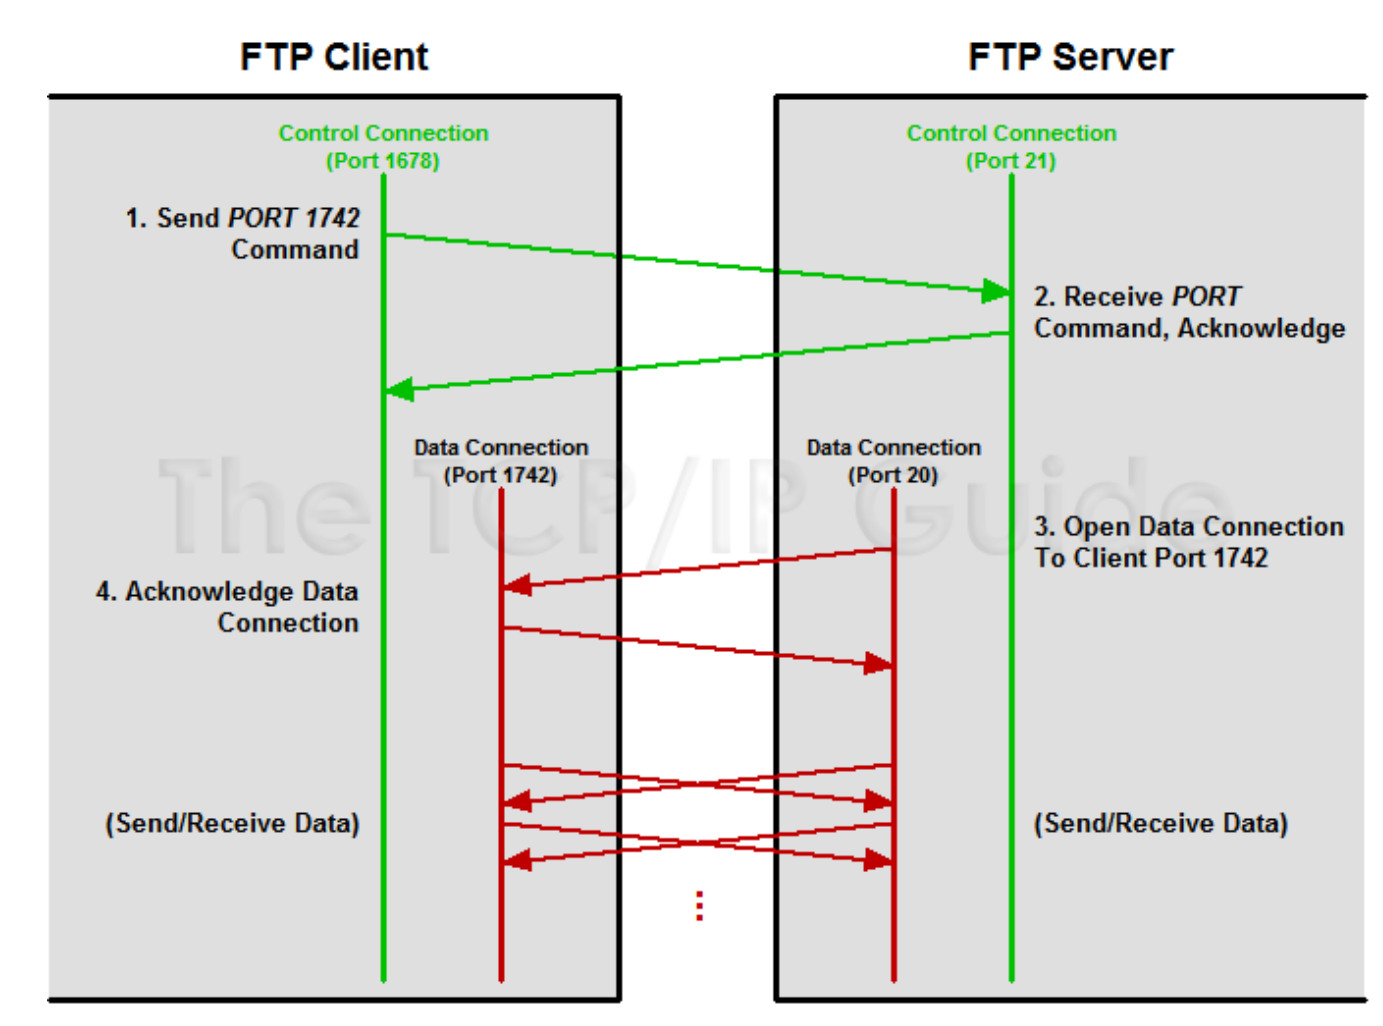
\includegraphics[width=0.75\linewidth]{figure/FTP.png}
    \caption{Diagramma di interazione}
    \label{fig:placeholder}
\end{figure}
Il diagramma di sequenza mostra l'invio del comando PORT da parte del client sulla connessione di controllo (es. porta 1678 verso porta 21 del server). Successivamente, il server apre la connessione dati (Porta 20 verso Porta 1742 del client) per iniziare il trasferimento effettivo.

\subsection{HTTP (HyperText Transfer Protocol)}
HTTP permette ad un host di \textbf{richiedere delle risorse}, chiamate
oggetti, ad un Web Server. Questi oggetti possono essere pagine
HTML o file multimediali di vario tipo. Per accedere a queste risorse
viene utilizzato un URL (Uniform Resource Locator). Esso è quindi il
protocollo alla base delle pagine Web, e segue l’architettura ClientServer. Le porte dedicate al protocollo sono:
\begin{itemize}
    \item \textbf{Porta 80} - lato server: è laporta da cui il server riceverà le richieste
    \item \textbf{Porta sorgente} - lato client: stabilita casualmente dal SO.
\end{itemize}
\subsubsection{URL} È composto da varie parti:
\begin{itemize}
    \item \textbf{Protocollo:} indica come deve avvenire la comunicazione (es: https://)
    \item \textbf{Nome di dominio:} Indica dove si trova la risorsa. È
associato a un indirizzo IP tramite DNS. (es: www.esempio.com)
    \item \textbf{Porta:} Indica su quale porta del server il browser deve collegarsi.
    \item \textbf{Path:} Indica quale risorsa si vuole sul server. (es: /cartella/pagina.it) 
    \item \textbf{Query stringhe:} Sono parametri aggiuntivi inviati al server usati per ricerche, per tracciare e per i login 
    \item \textbf{Frammento:} indica una parte specifica della pagina. Non viene inviato al server: serve solo al browser.
\end{itemize}
\end{document}